\documentclass[11pt]{article}
\usepackage[margin=1in]{geometry}
\usepackage{amsmath}
\usepackage{amssymb}
\usepackage{booktabs}
\usepackage{array}
\usepackage{tikz}
\usetikzlibrary{arrows.meta,positioning}

\title{3x3 Weight-Stationary Systolic Array Data Flow}
\author{}
\date{}

\begin{document}
\maketitle

\section*{1. What This RTL Is Actually Doing}

This note matches the \textbf{weight-stationary} RTL in:
\begin{itemize}
    \item \texttt{weightStationaryVariant/systolicArrayWeightStationary.sv}
    \item \texttt{weightStationaryVariant/multiplierBlockWeightStationary.sv}
    \item \texttt{weightStationaryVariant/weightLoader.sv}
    \item \texttt{weightStationaryVariant/dataOrchestratorWeightStationary.sv}
\end{itemize}

The dataflow has two phases:
\begin{enumerate}
    \item \textbf{Weight-load phase:} weights are pushed in from the top while \texttt{writeEnable = 1}. Each PE stores one weight in \texttt{weightReg}.
    \item \textbf{Compute phase:} activations enter from the left while \texttt{writeEnable = 0}. Each PE multiplies the activation by its stored weight, then adds into the vertical partial sum flowing downward.
\end{enumerate}

So this is not output-stationary. The stationary quantity is the \textbf{weight}.

\section*{2. PE-Level Operation}

Each PE implements:
\[
\texttt{bottomOut} \leftarrow \texttt{topIn} + \texttt{leftIn} \cdot \texttt{weightReg}
\]
and
\[
\texttt{rightOut} \leftarrow \texttt{leftIn}.
\]

That means:
\begin{itemize}
    \item activations move left to right,
    \item partial sums move top to bottom,
    \item weights stay stored inside the PEs after the load phase.
\end{itemize}

\section*{3. Matrix Mapping}

Let
\[
A =
\begin{bmatrix}
a_{00} & a_{01} & a_{02} \\
a_{10} & a_{11} & a_{12} \\
a_{20} & a_{21} & a_{22}
\end{bmatrix},
\qquad
B =
\begin{bmatrix}
b_{00} & b_{01} & b_{02} \\
b_{10} & b_{11} & b_{12} \\
b_{20} & b_{21} & b_{22}
\end{bmatrix}.
\]

In this RTL:
\begin{itemize}
    \item PE$(i,j)$ stores the weight $b_{ij}$ after the weight-load phase,
    \item row stream $i$ carries column $i$ of $A$ over time:
    \[
    a_{0i},\ a_{1i},\ a_{2i}.
    \]
\end{itemize}

At stream step $k$, the value currently entering row $i$ is $a_{ki}$. When that wavefront passes through column $j$, the column computes
\[
\sum_{i=0}^{2} a_{ki} b_{ij}.
\]

That is exactly
\[
C_{kj} = \sum_{i=0}^{2} a_{ki} b_{ij},
\]
which is standard matrix multiplication:
\[
C = AB.
\]

\section*{4. Why Column Streams of $A$ Still Produce Rows of $C$}

This is the subtle point.

Although row $0$, row $1$, and row $2$ receive:
\[
\text{column 0 of } A,\quad \text{column 1 of } A,\quad \text{column 2 of } A,
\]
they do \emph{not} represent three different output rows.

Instead, at stream index $k$, the three injected values are
\[
a_{k0},\ a_{k1},\ a_{k2},
\]
which together form \textbf{row $k$ of $A$}.

So one time step of the left-side injection reconstructs one full row of $A$ across the array rows. The fixed PE weights then dot that row with each column of $B$.

\section*{5. Explicit 3x3 PE Equations}

The stored weights are:
\[
\begin{array}{ccc}
\text{PE}(0,0): b_{00} & \text{PE}(0,1): b_{01} & \text{PE}(0,2): b_{02} \\
\text{PE}(1,0): b_{10} & \text{PE}(1,1): b_{11} & \text{PE}(1,2): b_{12} \\
\text{PE}(2,0): b_{20} & \text{PE}(2,1): b_{21} & \text{PE}(2,2): b_{22}
\end{array}
\]

Then the bottom outputs of the three columns produce:
\begin{align*}
C_{k0} &= a_{k0}b_{00} + a_{k1}b_{10} + a_{k2}b_{20}, \\
C_{k1} &= a_{k0}b_{01} + a_{k1}b_{11} + a_{k2}b_{21}, \\
C_{k2} &= a_{k0}b_{02} + a_{k1}b_{12} + a_{k2}b_{22},
\end{align*}
for $k = 0,1,2$.

Expanding all nine outputs:
\begin{align*}
C_{00} &= a_{00}b_{00} + a_{01}b_{10} + a_{02}b_{20}, \\
C_{01} &= a_{00}b_{01} + a_{01}b_{11} + a_{02}b_{21}, \\
C_{02} &= a_{00}b_{02} + a_{01}b_{12} + a_{02}b_{22}, \\
C_{10} &= a_{10}b_{00} + a_{11}b_{10} + a_{12}b_{20}, \\
C_{11} &= a_{10}b_{01} + a_{11}b_{11} + a_{12}b_{21}, \\
C_{12} &= a_{10}b_{02} + a_{11}b_{12} + a_{12}b_{22}, \\
C_{20} &= a_{20}b_{00} + a_{21}b_{10} + a_{22}b_{20}, \\
C_{21} &= a_{20}b_{01} + a_{21}b_{11} + a_{22}b_{21}, \\
C_{22} &= a_{20}b_{02} + a_{21}b_{12} + a_{22}b_{22}.
\end{align*}

\section*{6. Structural Picture}

\begin{center}
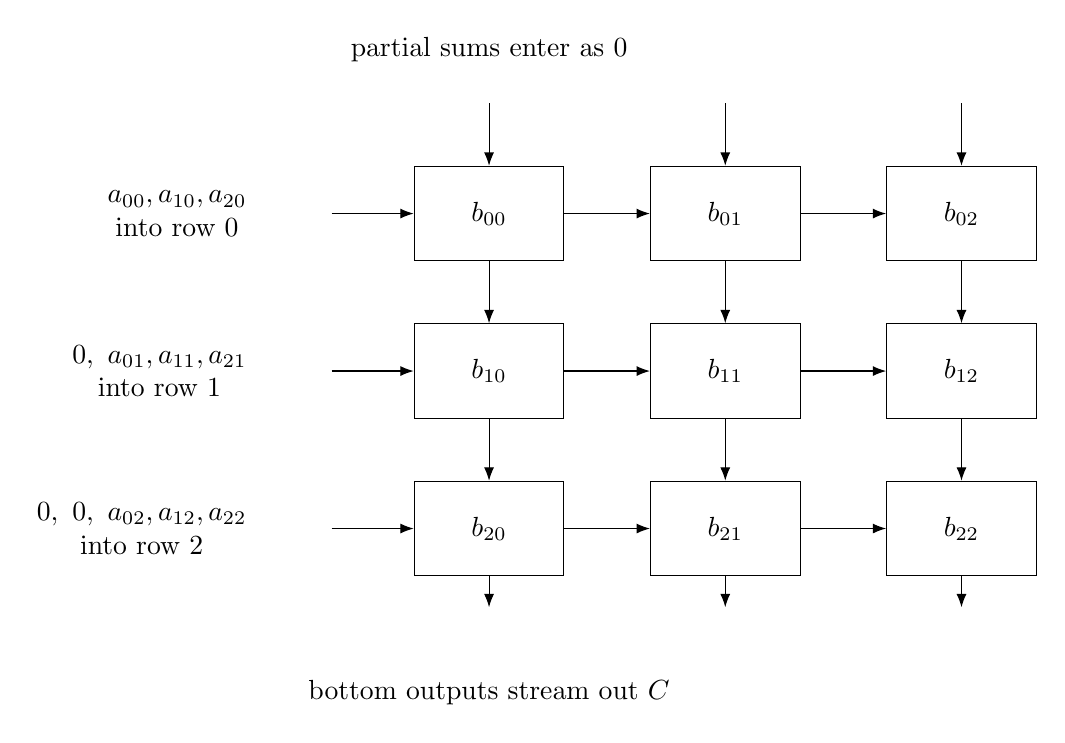
\begin{tikzpicture}[
    pe/.style={draw, minimum width=1.9cm, minimum height=1.2cm, align=center},
    lbl/.style={align=center},
    >=Latex
]

\node[pe] (p00) at (0,0) {$b_{00}$};
\node[pe] (p01) at (3,0) {$b_{01}$};
\node[pe] (p02) at (6,0) {$b_{02}$};

\node[pe] (p10) at (0,-2) {$b_{10}$};
\node[pe] (p11) at (3,-2) {$b_{11}$};
\node[pe] (p12) at (6,-2) {$b_{12}$};

\node[pe] (p20) at (0,-4) {$b_{20}$};
\node[pe] (p21) at (3,-4) {$b_{21}$};
\node[pe] (p22) at (6,-4) {$b_{22}$};

\node[lbl, left=2.0cm of p00] {$a_{00},a_{10},a_{20}$\\into row 0};
\node[lbl, left=2.0cm of p10] {$0,\ a_{01},a_{11},a_{21}$\\into row 1};
\node[lbl, left=2.0cm of p20] {$0,\ 0,\ a_{02},a_{12},a_{22}$\\into row 2};

\node[lbl, above=1.2cm of p00] {partial sums enter as $0$};
\node[lbl, below=1.2cm of p20] {bottom outputs stream out $C$};

\draw[->] (-2.0,0) -- (p00);
\draw[->] (-2.0,-2) -- (p10);
\draw[->] (-2.0,-4) -- (p20);

\draw[->] (p00) -- (p01);
\draw[->] (p01) -- (p02);
\draw[->] (p10) -- (p11);
\draw[->] (p11) -- (p12);
\draw[->] (p20) -- (p21);
\draw[->] (p21) -- (p22);

\draw[->] (0,1.4) -- (p00);
\draw[->] (3,1.4) -- (p01);
\draw[->] (6,1.4) -- (p02);

\draw[->] (p00) -- (p10);
\draw[->] (p10) -- (p20);
\draw[->] (p01) -- (p11);
\draw[->] (p11) -- (p21);
\draw[->] (p02) -- (p12);
\draw[->] (p12) -- (p22);

\draw[->] (p20) -- ++(0,-1.0);
\draw[->] (p21) -- ++(0,-1.0);
\draw[->] (p22) -- ++(0,-1.0);

\end{tikzpicture}
\end{center}

The labels inside the PEs are the weights that remain stationary during computation.

\section*{7. Timing: Weight Loading}

The weight loader runs first while \texttt{writeEnable = 1}. During this phase:
\begin{itemize}
    \item top inputs carry weight values,
    \item left inputs are effectively zero,
    \item each PE captures \texttt{topIn[WIDTH-1:0]} into \texttt{weightReg}.
\end{itemize}

The weights are sent \emph{downward} through the array during loading, so each column gets filled from top to bottom over several cycles.

Conceptually, column $j$ is loaded so that:
\[
\begin{array}{c}
\text{PE}(0,j) \gets b_{0j} \\
\text{PE}(1,j) \gets b_{1j} \\
\text{PE}(2,j) \gets b_{2j}
\end{array}
\]
once the load phase finishes.

\section*{8. Timing: Compute Phase and Stagger}

After the weights are loaded, \texttt{writeEnable} goes low and the activation stream begins.

The orchestrator staggers the rows:
\[
\text{row 0: } a_{00},\ a_{10},\ a_{20}
\]
\[
\text{row 1: } 0,\ a_{01},\ a_{11},\ a_{21}
\]
\[
\text{row 2: } 0,\ 0,\ a_{02},\ a_{12},\ a_{22}
\]

So yes: the row below arrives one cycle later, and the next row one more cycle later.

Equivalently, the value $a_{ki}$ is injected into row $i$ at time
\[
t = t_0 + i + k,
\]
where $t_0$ is the start of the compute phase.

Then it takes one more cycle per PE to move to the right, so $a_{ki}$ reaches PE$(i,j)$ at
\[
t = t_0 + i + j + k.
\]

That is the diagonal wavefront.

\section*{9. One Full Example: How $C_{12}$ Is Formed}

Take column $j=2$ and output row $k=1$.

We want:
\[
C_{12} = a_{10}b_{02} + a_{11}b_{12} + a_{12}b_{22}.
\]

During the compute phase:
\begin{itemize}
    \item row 0 contributes $a_{10}$ and PE$(0,2)$ multiplies by $b_{02}$,
    \item row 1 contributes $a_{11}$ and PE$(1,2)$ multiplies by $b_{12}$,
    \item row 2 contributes $a_{12}$ and PE$(2,2)$ multiplies by $b_{22}$.
\end{itemize}

These three products are accumulated down column 2 as the partial sum travels downward, and the finished value exits the bottom of that column.

\section*{10. What the Bottom Outputs Mean}

The array output in \texttt{systolicArrayWeightStationary.sv} is:
\[
\texttt{result[j]} = \texttt{verticalData[N][j]}.
\]

So each bottom output corresponds to one output column:
\begin{itemize}
    \item bottom output 0 streams values for column 0 of $C$,
    \item bottom output 1 streams values for column 1 of $C$,
    \item bottom output 2 streams values for column 2 of $C$.
\end{itemize}

Because of the skew, the values do not all appear at once. They emerge over time in a staggered pattern.

\section*{11. Short Summary}

\begin{itemize}
    \item This design is weight-stationary because each PE stores one weight $b_{ij}$.
    \item The left-going streams are staggered activation values from $A$.
    \item At stream step $k$, the three row injections form row $k$ of $A$ across the array rows.
    \item Each column of PEs computes one dot product with a column of $B$.
    \item The bottom outputs therefore stream the entries of $C = AB$.
\end{itemize}

\end{document}
